\documentclass{article}
\usepackage[utf8]{inputenc}
\usepackage{hyperref}
\usepackage{pdfrender,xcolor}
\usepackage{graphicx}



\usepackage{amsmath,amssymb,amsthm}
\usepackage{mathtools,graphicx,tikz-cd}
\usepackage{blindtext}
\usepackage[margin = 1.25 in]{geometry}
\usepackage{enumitem}

\usepackage{fancyhdr,accents,lastpage}
\pagestyle{fancy}
\setlength{\headheight}{25pt}

\newtheorem{theorem}{Theorem}[section]
\newtheorem{corollary}{Corollary}[theorem]
\newtheorem{lemma}[theorem]{Lemma}

\theoremstyle{definition}
\newtheorem{definition}{Definition}[section]

\theoremstyle{remark}
\newtheorem*{remark}{Remark}
\newtheorem{exercise}{Exercise}
\newtheorem{example}{Example}[definition]


\DeclareMathOperator{\ab}{ab}
\DeclareMathOperator{\area}{area}
\DeclareMathOperator{\Aut}{Aut}
\DeclareMathOperator{\BGL}{BGL}
\DeclareMathOperator{\Br}{Br}
\DeclareMathOperator{\card}{card}
\DeclareMathOperator{\ch}{ch}
\DeclareMathOperator{\Char}{char}
\DeclareMathOperator{\CHur}{CHur}
\DeclareMathOperator{\Cl}{Cl}
\DeclareMathOperator{\coker}{coker}
\DeclareMathOperator{\Conf}{Conf}
\DeclareMathOperator{\disc}{disc}
\DeclareMathOperator{\End}{End}
\DeclareMathOperator{\et}{\text{\'et}}
\DeclareMathOperator{\Fix}{Fix}
\DeclareMathOperator{\Gal}{Gal}
\DeclareMathOperator{\GL}{GL}
\DeclareMathOperator{\Hom}{Hom}
\DeclareMathOperator{\Hur}{Hur}
\DeclareMathOperator{\im}{im}
\DeclareMathOperator{\Ind}{Ind}
\DeclareMathOperator{\Inn}{Inn}
\DeclareMathOperator{\Irr}{Irr}
\DeclareMathOperator{\lcm}{lcm}
\DeclareMathOperator{\Mor}{Mor}
\DeclareMathOperator{\ord}{ord}
\DeclareMathOperator{\Out}{Out}
\DeclareMathOperator{\Perm}{Perm}
\DeclareMathOperator{\PGL}{PGL}
\DeclareMathOperator{\Pin}{Pin}
\DeclareMathOperator{\PSL}{PSL}
\DeclareMathOperator{\rad}{rad}
\DeclareMathOperator{\sgn}{sgn}
\DeclareMathOperator{\SL}{SL}
\DeclareMathOperator{\SO}{SO}
\DeclareMathOperator{\Sp}{Sp}
\DeclareMathOperator{\Spec}{Spec}
\DeclareMathOperator{\Spin}{Spin}
\DeclareMathOperator{\St}{St}
\DeclareMathOperator{\Surj}{Surj}
\DeclareMathOperator{\Syl}{Syl}
\DeclareMathOperator{\tame}{tame}
\DeclareMathOperator{\Tr}{Tr}

\newcommand{\eps}{\varepsilon}
\newcommand{\QED}{\hspace{\stretch{1}} $\blacksquare$}
\renewcommand{\AA}{\mathbb{A}}
\newcommand{\CC}{\mathbb{C}}
\newcommand{\EE}{\mathbb{E}}
\newcommand{\FF}{\mathbb{F}}
\newcommand{\HH}{\mathbb{H}}
\newcommand{\NN}{\mathbb{N}}
\newcommand{\OO}{\mathbb{O}}
\newcommand{\PP}{\mathbb{P}}
\newcommand{\QQ}{\mathbb{Q}}
\newcommand{\RR}{\mathbb{R}}
\newcommand{\ZZ}{\mathbb{Z}}
\newcommand{\bfm}{\mathbf{m}}
\newcommand{\mcA}{\mathcal{A}}
\newcommand{\mcC}{\mathcal{C}}
\newcommand{\mcG}{\mathcal{G}}
\newcommand{\mcH}{\mathcal{H}}
\newcommand{\mcM}{\mathcal{M}}
\newcommand{\mcN}{\mathcal{N}}
\newcommand{\mcO}{\mathcal{O}}
\newcommand{\mcP}{\mathcal{P}}
\newcommand{\mcQ}{\mathcal{Q}}
\newcommand{\mfa}{\mathfrak{a}}
\newcommand{\mfb}{\mathfrak{b}}
\newcommand{\mfI}{\mathfrak{I}}
\newcommand{\mfM}{\mathfrak{M}}
\newcommand{\mfm}{\mathfrak{m}}
\newcommand{\mfo}{\mathfrak{o}}
\newcommand{\mfO}{\mathfrak{O}}
\newcommand{\mfP}{\mathfrak{P}}
\newcommand{\mfp}{\mathfrak{p}}
\newcommand{\mfq}{\mathfrak{q}}
\newcommand{\mfz}{\mathfrak{z}}
\newcommand{\AGL}{\mathbb{A}\GL}
\newcommand{\Qbar}{\overline{\QQ}}
\renewcommand{\qedsymbol}{$\blacksquare$}

%\pdfrender{StrokeColor=black,TextRenderingMode=2,LineWidth=0.5pt}

%\lhead{\pdfrender{StrokeColor=black,TextRenderingMode=2,LineWidth=0.5pt}Planar Geometry} 
%\chead{\pdfrender{StrokeColor=black,TextRenderingMode=2,LineWidth=0.5pt}Math Club}
%\rhead{\pdfrender{StrokeColor=black,TextRenderingMode=2,LineWidth=0.5pt}Winter 2021}
\lhead{Planar Geometry}
\chead{Math Club}
\rhead{Winter 2021}


\begin{document}
\section{Introduction}
Despite that planar geometry plays a less important role in higher level of math, it is intrinsically beautiful and has prepossessed a lot of famous mathematicians. Recorded in the Euclid's \emph{Elements}, planar geometry was a protagonist of the math community dating back to Ancient Greece. Even if nowadays there're less ongoing research in planar geometry, the subject still fascinates math people and occasionally appears in the Putnam contest. In this handout, we introduce the Euclid's Postulates and present several problems in planar geometry. Some of them are less in the spirit of Euclid, being based on algebraic or combinatorial considerations. Here “imagination is more important than knowledge’’ (A. Einstein).

\section{Resources}
The problems above and below are shamelessly ripped from the books \textit{Putnam and Beyond} by Andreescu and Gelca and \textit{Problem Solving Strategies} by Arthur Engel. We also stole some problems from the Putnam competition. Many other problem solving books have induction sections as well. These problems are arranged roughly in order of difficulty, but difficulty is relative to each person so take it with a grain of salt.

\section{Euclid's Postulates} 
\begin{itemize}
    \item A straight line segment can be drawn joining any two points.
    \item Any straight line segment can be extended indefinitely in a straight line.
    \item Given any straight lines segment, a circle can be drawn having the segment as radius and one endpoint as center.
    \item All right angles are congruent.
    \item If two lines are drawn which intersect a third in such a way that the sum of the inner angles on one side is less than two Right Angles, then the two lines inevitably must intersect each other on that side if extended far enough. This postulate is equivalent to what is known as the Parallel Postulate.
\end{itemize}

\section{Easy}
\begin{exercise}
Prove the Pythagorean Theorem. How do you tell whether a triangle is acute, right, or obtuse?  
\end{exercise}
\begin{exercise}
Prove that the midpoints of the sides of a quadrilateral form a parallelogram.
\end{exercise}

\begin{exercise}
In triangle $ABC$, $AB = 13$, $BC = 14$, and $CA = 15$. Distinct points $D, E,$ and $F$ lie on segments $BC, CA,$ and $DE$, respectively, such that $AD \perp BC$, $DE \perp AC$, and $AF \perp BF$. The length of segment $DF$ can be written as $mn$ , where $m$ and $n$ are relatively prime positive integers. What is $m + n$?
\end{exercise}

\begin{exercise}
A straight line cuts the asymptotes of a hyperbola in points $A$ and $B$ and the curve in points $P$ and $Q$. Prove that $AP = BQ$.   
\end{exercise}

\begin{exercise}[2010 B2]
Given $A$, $B$, and $C$ are noncollinear points in the plane with integer coordinates such that the distances $AB$, $AC$, and $BC$ are integers, what is the smallest possible value of $AB$?
\end{exercise}

\begin{exercise}
In the figure shown below, circle $B$ is tangent to circle $A$ at $X$, circle $C$ is tangent to circle $A$ at $Y$ , and circles $B$ and $C$ are tangent to each other. If $AB = 6, AC = 5,$ and $BC = 9$, what is $AX$?
\begin{figure}[hbt!]
\label{fig:aa}
\small
\centering
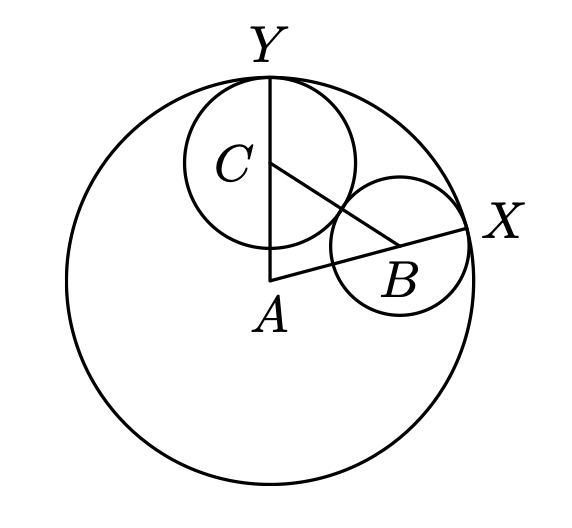
\includegraphics[scale = 0.4]{1.png}
\end{figure}
\end{exercise}

\section{Medium}

\begin{exercise}
Let $ABCD$ be a convex quadrilateral, and define $P_1, P_2, P_3, P_4, P_5,$ and $P_6$ to be the midpoints of line segments $AB, BC, CD, DA, AC,$ and $BD$ respectively. Prove that lines $P_{1}P_{3}$, $P_{2}P_{4}$, and $P_{5}P_{6}$ all intersect in a single point.
\end{exercise}

\begin{exercise}[2012 A1]
Let $d_{1}, d_{2}, \ldots, d_{12}$ be real numbers in the open interval $(1, 12)$. Show that there exist distinct indices $i, j, k$ such that $d_{i}$,$d_{j},d_{k}$ are the side lengths of an acute triangle.
\end{exercise}

\begin{exercise}[1998 B2]
Given a point $(a, b)$ with $0 < b < a$, determine the minimum perimeter of a triangle with one vertex at $(a, b)$, one on the $x$-axis, and one on the line $y = x$. You may assume that a triangle of minimum perimeter exists.
\end{exercise}

\begin{exercise}[2015 A1]
Let $A$ and $B$ be points on the same branch of the hyperbola $xy = 1$. Suppose that $P$ is a point lying between $A$ and $B$ on this hyperbola, such that the area of the triangle $APB$ is as large as possible. Show that the region bounded by the hyperbola and the chord $AP$ has the same area as the region bounded by the hyperbola and the chord $PB$.
\end{exercise}

\begin{exercise}[1992 CMO]
A convex quadrilateral $ABCD$ is inscribed in a circle with center $O$. The diagonals $AC, BD$ of $ABCD$ meet at $P$. Circumcircles of $ABP$ and $CDP$ meet at $P$ and $Q$ ($O, P, Q$ are pairwise distinct). Show that the angle of $OQP$ is $90^{\circ}$. 
\end{exercise}

\section{Hard}
\begin{exercise}
Acute-angled triangle $ABC$ is inscribed into circle $\Omega$. Lines tangent to $\Omega$ at $B$ and $C$ intersect at $P$. Points $D$ and $E$ are on $AB$ and $AC$ such that $PD$ and $PE$ are perpendicular to $AB$ and $AC$ respectively. Prove that the orthocenter of triangle $ADE$ is the midpoint of $BC$.
\end{exercise}

\begin{exercise}[2017 B5]
A line in the plane of a triangle $T$ is called an equalizer if it divides $T$ into two regions having equal area and equal perimeter. Find positive integers $a > b > c$, with a as small as possible, such that there exists a triangle with side lengths $a, b, c$ that has exactly two equalizers.
\end{exercise}

\begin{exercise}[2018 A6]
Suppose that $A$, $B$, $C$, and $D$ are distinct points, no three of which lie on a line, in the Euclidean plane. Show that if the squares of the lengths of the line segments $AB$, $AC$, $AD$, $BC$, $BD$, and $CD$ are rational numbers, then the quotient
\[\frac{\area(\Delta ABC)}{\area(\Delta ABD)}\]
is a rational number.
\end{exercise}

\newpage
\section{Hint}
\begin{itemize}
    \item Various proofs 
    \item Use coordinates 
    \item Draw the picture 
    \item Write down the standard form of a hyperbola 
	\item First guess the answer, and then prove that no smaller values are possible
	\item The intersection points are important 
	\item Make use of the result of Exercise 2 
	\item What's the property for an acute triangle 
	\item Use reflections 
    \item Shoelace's formula, and then AM-GM 
    \item Connect $AO$, $AQ$, $DO$, and $DQ$ 
\end{itemize}

\newpage
\section{Appendix}
Here are important things in middle/high school Olympiads competitions. Some of the results might be used to solve planar geometry problems in the Putnam contest.    
\begin{itemize}
    \item Properties of parallelism, orthogonality, similar triangles, and cyclic quadrilateral   
    \item The Law of Sines, The Law of Cosines, Heron's Formula
    \item Intersecting Chords Theorem, Tangent Secant Theorem 
    \item Pythagorean Theorem 
    \item Geometric Mean Theorem 
    \item Stewart's Theorem 
    \item Menelaus's Theorem, Ceva's Theorem 
    \item Ptolemy's Theorem, Simson's Theorem 
    \item The incenter, circumcenter, centroid, orthocenter, and escenter of a triangle 
    \item Radical axis of two circles 
    \item Euler's Theorem, Fermat Point, Nine-point circle 
    \item Coordinate geometry: line, circle, parabola, ellipse, hyperbola, and second definitions  
\end{itemize}
\end{document}
 